\lesson{Atomic Structure and the Periodic Table}
The main thing to understand from the previous section is that there are four quantized values that
describe an electron in an atom. Quantized means that the values are restricted to certain discrete
values.

\begin{tabular-custom}{|l|l|l|l|l|}{Values and letters for the secondary quantum number}
    Value of $\ell$ & 0 & 1 & 2 & 3 \\ \hline
    Letter designation & s & p & d & f \\ \hline
    Name designation & \textbf{s}harp & \textbf{p}rincipal & \textbf{d}iffuse & \textbf{f}undamental \\ \hline
\end{tabular-custom}

\subsection{Electron Orbitals}
\begin{bulleted-list}
    \item Bohr's theory was based on the idea of an electron travelling in a orbit path. A
        more modern view is that of an electron \textbf{orbital}
        \footnote{
            \textbf{Orbital:} a region of space around the nucleus where an electron is likely
            to be found.
        }
    \item As we move from focusing on the energy of electrons to focusing on their position, the
        terminology will change from using principal energy level to \textbf{shell}
        \footnote{
            \textbf{Shell:} main energy level; the shell number is given by the principal quantum
            number $n$
        }
        , and from energy sublevel to \textbf{subshell}.
        \footnote{
            \textbf{Subshell:} orbiatls of different shapes and energies, given by the secondary
            quantum number $\ell$
        }
    \item Chemists usually use the number for the main energy level and a letter designation
        for the energy sublevel. For example, a $1s$ orbital, a $2p$ orbital, a $3d$ orbital,
        or a $4f$ orbital in that energy sublevel can be specified.
\end{bulleted-list}

\begin{tabular-custom}{|l|l|}{Orbits and orbitals}
    Orbits & Orbitals \\ \hline
    2-D path & 3-D region in space \\ \hline
    Fixed distance from nucleus & Variable distance from nucleus \\ \hline
    Circular or elliptical path & No path; varied shape of region \\ \hline
    $2n^2$ electrons per orbit & 2 electrons per orbital \\ \hline
\end{tabular-custom}

\subsection{Creating Energy-Level Diagrams}
\begin{bulleted-list}
    \item The previous energy level diagrams only included the principal quantum number. Now,
        it also use the secondary quantum number
    \item In Figure \ref{fig:energy-level-diagram}, as the atoms become larger and the main
        energy levels become closer together, some sublevels start to overlap in energy
    \item The energy of an electron increases with an increasing value of the principal quantum
        number. For a given value of $n$, the sublevels increase in energy, in order s < p < d < f
\end{bulleted-list}

\begin{figure}[ht!]
    \centering
    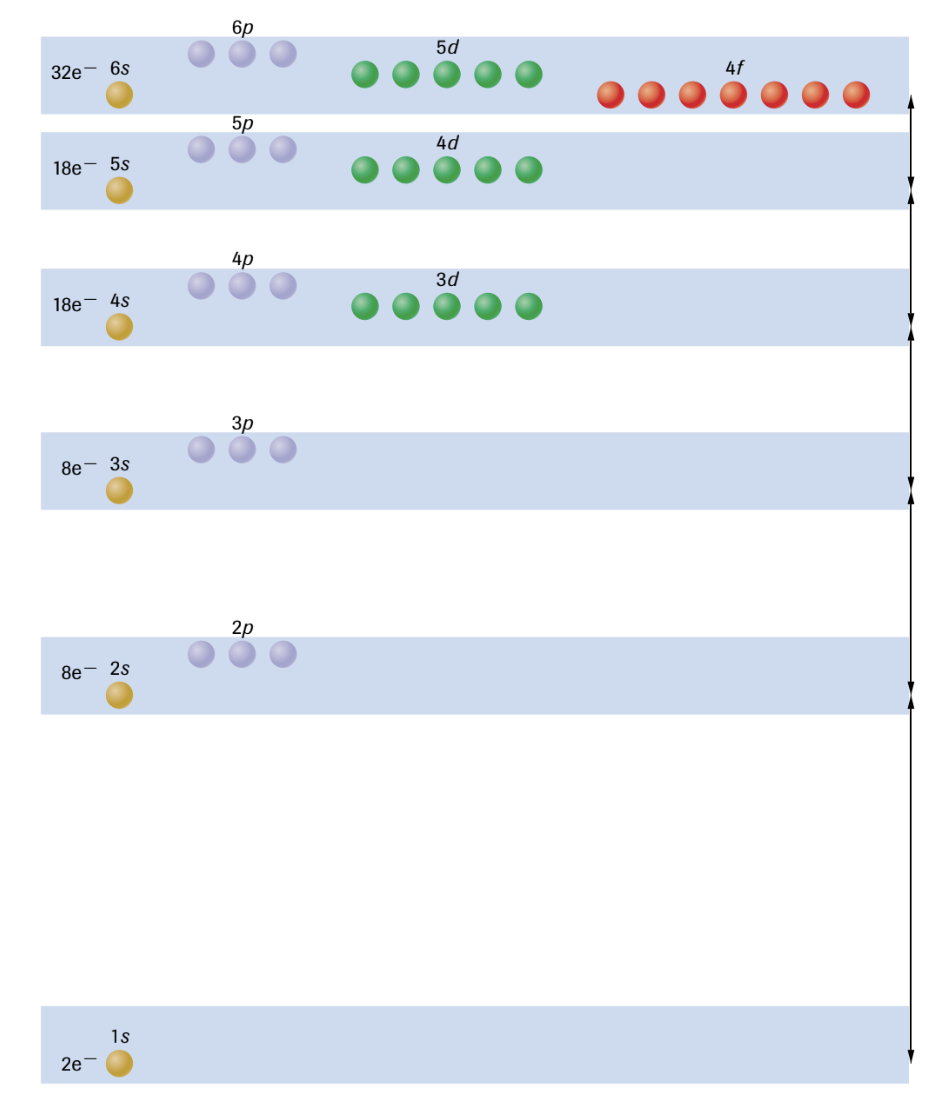
\includegraphics[width=0.7 \textwidth]{../figures/energy-level-diagram.png}
    \caption{Diagram of relative energies of electrons in various orbitals. Each orbital (circle)
            can potentially contain up to two electrons.}
    \label{fig:energy-level-diagram}
\end{figure}

\begin{bulleted-list}
    \item Show an electron in an orbital by placing an up arrow or a down arrow, or both to represent
        an electron pair. According to the \textbf{Pauli exclusion principle}
        \footnote{
            \textbf{Pauli exclusion principle:} no two electrons in an atom can have the same
            four quantum numbers.
        }
        , the two electrons cannot point in the same direction
    \item An energy sublevel must be filled before moving onto the next higher energy sublevel,
        according to the \textbf{Aufbau principle}
        \footnote{
            \textbf{Aufbau principle:} ``aufbau'' is German for building up; each electron is
            added to the lowest energy orbital available in an atom or ion.
        }.
        See Figure \ref{fig:aufbau-principle}.
    \item Spread out the electrons as much as possible horizontally before doubling up any
        pair of electrons, according to \textbf{Hund's rule}
        \footnote{
            \textbf{Hund's rule:} one electron occupies each of several orbitals at the same
            energy before a second electron can occupy the same orbital.
        }
    \item In Figure \ref{fig:energy-level-diagrams-lithium-carbon-fluorine}, for (a), according
        to the Aufbau principle, the 1s orbital must be filled up first before moving onto the
        2s orbital. For (b) and (c), according to Hund's rule, all of the orbitals must have one electron
    \item As you move across the periodic table, each atom has one more electron than the previous.
        Because the electrons are added sequentially to the lowest energy orbital available
        (Aufbau principle), the elements can be classified by the sublevel currently being filled.
        See Figure \ref{fig:electron-configurations}
\end{bulleted-list}

\begin{figure}[ht!]
    \centering
    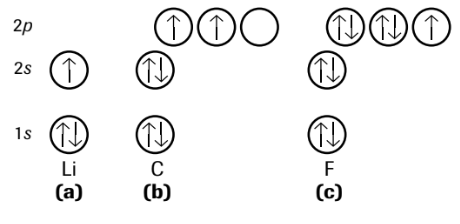
\includegraphics[width=0.4 \textwidth]{../figures/energy-level-diagrams-lithium-carbon-fluorine.png}
    \caption{Energy-level diagrams for lithium, carbon, and fluorine atoms}
    \label{fig:energy-level-diagrams-lithium-carbon-fluorine}
\end{figure}

\begin{figure}[ht!]
    \centering
    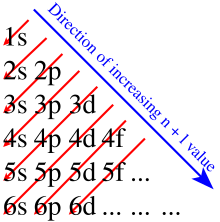
\includegraphics[width=0.2 \textwidth]{../figures/aufbau-principle.png}
    \caption{Start and the top and move in the direction of the arrows for the orbiatls}
    \label{fig:aufbau-principle}
\end{figure}

\newpage

\begin{figure}[ht!]
    \centering
    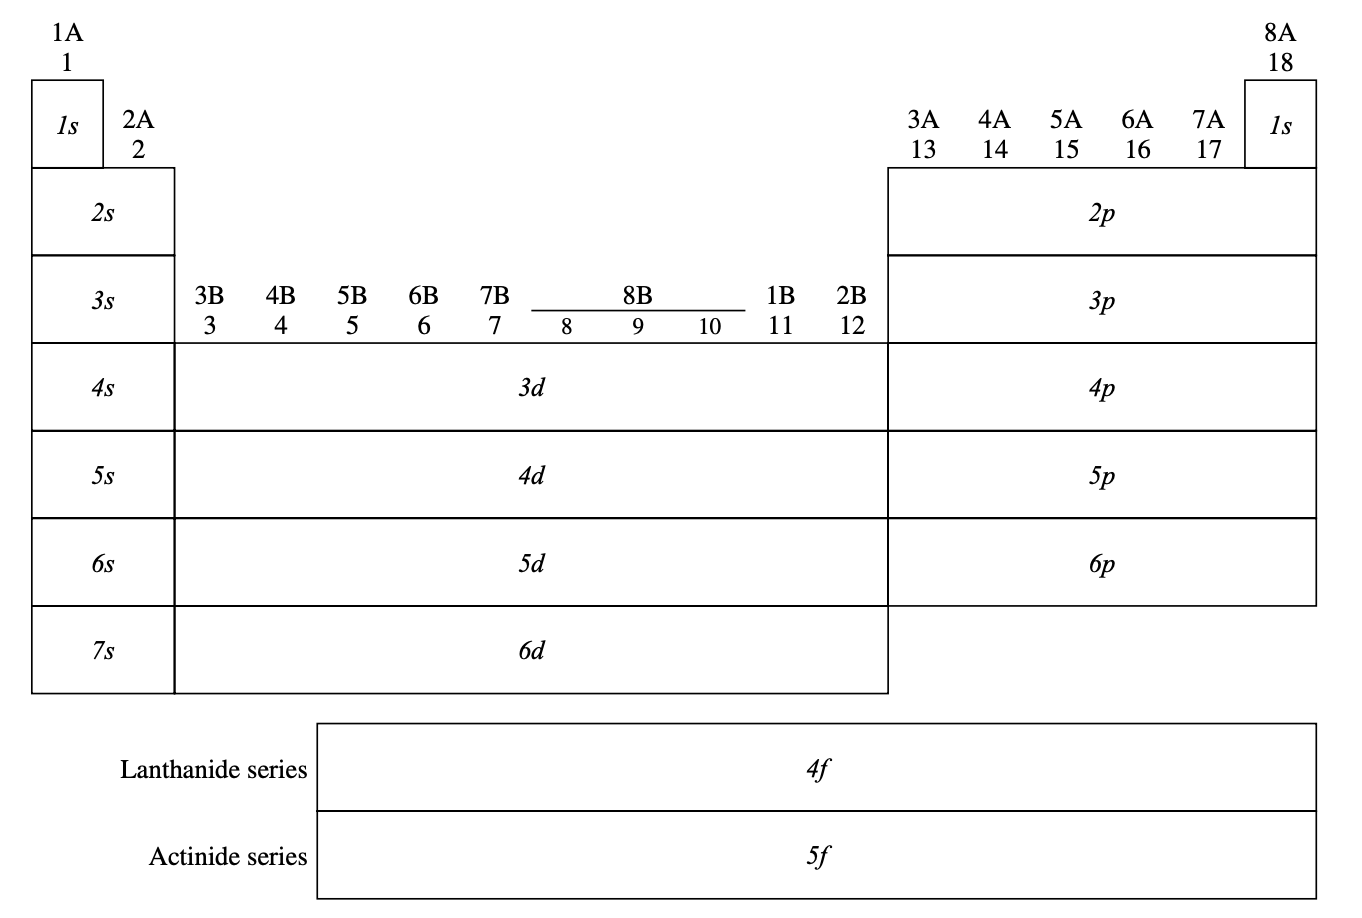
\includegraphics[width=0.6 \textwidth]{../figures/electron-configurations.png}
    \caption{Classification of elements by the sublevels that are being filled}
    \label{fig:electron-configurations}
\end{figure}

\begin{sample}{Draw the energy-level diagram for an iron atom.}
    \begin{figure}[ht!]
        \centering
        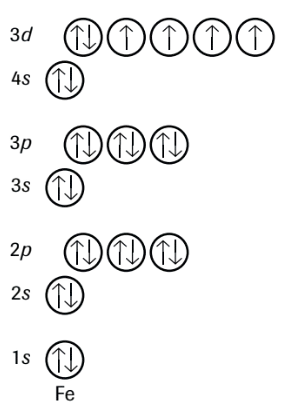
\includegraphics[width=0.2 \textwidth]{../figures/energy-level-diagram-iron.png}
    \end{figure}
\end{sample}

\subsection{Creating Energy-Level Diagrams for Anions and Cations}
\begin{bulleted-list}
    \item For anions, simply add the corresponding number of electrons to the configuration
    \item For cations, remove the number of electrons from the orbitals with the \textbf{highest}
        principal quantum number, because they represent the valence shell
\end{bulleted-list}

\begin{sample}{Draw the energy-level diagram for the sulfide ion.}
    Sulfur is an anion, so we add the corresponding 2 electrons to the energy-level diagram.
    \begin{figure}[ht!]
        \centering
        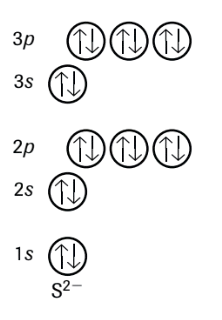
\includegraphics[width=0.15 \textwidth]{../figures/energy-level-diagram-sulfide-ion.png}
    \end{figure}
\end{sample}

\begin{sample}{Draw the energy-level diagram for the zinc ion.}
    Zinc is a cation, so we remove the corresponding 2 electrons from the orbitals with the highest
    principal quantum number, in this case being 4s.
    \begin{figure}[ht!]
        \centering
        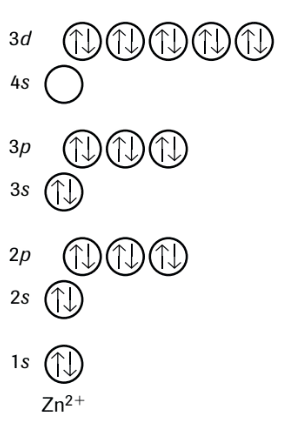
\includegraphics[width=0.15 \textwidth]{../figures/energy-levecl-diagram-zinc-ion.png}
    \end{figure}
\end{sample}

\begin{sample}{State the names of the three main rules/principles used to construct an energy-level
    diagram. Briefly describe each of these in your own words.}
    The three rules/princples are
    \begin{enum-alph}
        \item Pauli exclusion principle: no two electrons can have the same four quantum numbers
        \item Aufbau principle: each electron is added from the lowest energy orbital available
        \item Hund's rule: all of the orbitals must have a single electron before doubling up
    \end{enum-alph}
\end{sample}

\begin{sample}{How can the periodic table be used to help complete energy-level diagarams?}
    As you move across the periodic table, each atom has one more electron than the previous.
    Because the electrons are added sequentially to the lowest energy level (Aufbau principle),
    the atom can be classified by the current sublevel being filled.
\end{sample}

\begin{sample}{Complete the electron energy-level diagrams for
        \begin{enum-alph}
            \item phosphorus atom
            \item potassium atom
            \item manganese atom
            \item nitride ion
            \item bromide ion
            \item cadmium ion
        \end{enum-alph}
    }
    Watch out for the word ion.
\end{sample}

\begin{sample}{
        \begin{enum-alph}
            \item Complete the electron energy-level diagrams for a potassium ion and a chloride ion
            \item Which noble gas atom has the same electron energy-level diagram as these ions?
        \end{enum-alph}
    }
    \begin{enum-alph}
        \item The potassium ion is a cation and the chloride ion is an anion
        \item This is asking the same question as ``which element is isoelectronic to the potassium
            cation and which element is isoelectronic to the chloride anion?''. Argon is isoelectronic
            to both the potassium cation and the chloride anion
    \end{enum-alph}
\end{sample}

\subsection{Electron Configurations}
An electron configuration is a listing of the number and kinds of electrons in order of increasing energy.
You can also shorthand it by writing the noble gas from the period above it first in square
followed by the rest of the configuration in the period.

\begin{sample}{Write the electron configuration for the chlorine atom.}
    Cl: $\ch{1s^2 2s^2 3s^2 3p^5}$, or $\ch{[Ne] 3s^2 3p^5}$
\end{sample}

\begin{sample}{Identify the atoms that have the following electron configurations:
        \begin{enum-alph}
            \item $\ch{1s^2 2s^2 2p^6 3s^2 3p^6 4s^2 3d^10 4p^5}$
            \item $\ch{1s^2 2s^2 2p^6 3s^2 3p^6 4s^2 3d^10 4p^5 5s^2 4d^5}$
            \item $\ch{1s^2 2s^2}$
            \item $\ch{1s^2 2s^2 2p^5}$
            \item $\ch{1s^2 2s^2 2p^6 3s^1}$
            \item $\ch{1s^2 2s^2 2p^6 3s^2 3p^4}$
        \end{enum-alph}
    }
    \begin{enum-alph}
        \item Br, bromine
        \item Tc, technetium
        \item Be, beryllium
        \item F, fluorine
        \item Na, sodium
        \item S, sulfur
    \end{enum-alph}
\end{sample}

\begin{sample}{Write the shorthand electron electron configuration for the lead atom and
    the lead(II) ion.}

    Pb: $\ch{[Xe] 6s^2 4f^14 5d^10 6p^2}$

    $\ch{Pb^{2+}}$: $\ch{[Xe] 6s^2 5d^10}$
\end{sample}

\begin{sample}{Write the full electron configurations for a fluoride ion and a sodium ion.}

    $\ch{F^-}$: $\ch{1s^2 2s^2 2p^6}$

    $\ch{Na^+}$: $\ch{1s^2}$
\end{sample}

\begin{sample}{A fluoride ion and neon atom are theoretically described as isoelectronic. State
    the meaning of this term.}
    Isoelectronic means two atoms that have the same number of electrons and theoretically the
    same electron configuration.
\end{sample}

\subsection{Explaining the Periodic Table}
\begin{bulleted-list}
    \item The four quantum numbers were developed using experimental studies of atomic spectra
        and the experimentally determined arrangement of elements in the periodic table. It is no
        coincidence that the maximum number of electrons in the s, p, d, and f orbitals correspond
        exactly to the number of columns of elements in the s, p, d, and f blocks in the periodic
    \item \textbf{Representative elements}
        \footnote{
            \textbf{Representative elements:} the metals and nonmetals in groups 1-2 and 13-18.
            In other words, the s and p blocks.
        }
        have their properties much more precisely defined because
        they can be explained with having s and p orbitals
    \item \textbf{Transition elements}
        \footnote{
            \textbf{Transition elements:} the metals in groups 3-12; elements filling d orbitals with
            electrons.
        }
        can now be explained as having d orbitals, hence why they
        can store so many electrons in some sublevels
    \item The lathanides and actinides can also be explained as a series of elements filling an f
        energy level. The f block of elements is 14 elements wide, as expected by filling 7 orbitals
        with 14 electrons
\end{bulleted-list}

\begin{table}[!ht]
    \centering
    \caption{Electron subshells and the periodic table}
    \arrayrulecolor{black}            % table border color
    \begin{tabular}{|l|c|l l l l l|}
        \hline
        \rowcolor{HeaderColor}
        Period & \# of elements & groups: & 1-2 & 13-18 & 3-12 & - \\
        \rowcolor{HeaderColor}
               & & orbitals: & s & p & d & f \\ \hline
        Period 1 & 2 & & 2 & & & \\ \hline
        Period 2 & 8 & & 2 & 6 & & \\ \hline
        Period 3 & 18 & & 2 & 6 & 10 & \\ \hline
        Period 4-5 & 18 & & 2 & 6 & 10 & \\ \hline
        Period 6-7 & 18 & & 2 & 6 & 10 & 14 \\ \hline
    \end{tabular}
\end{table}

\subsection{Explaining Ion Charges}
Many of the transition metals are multivalent, and this theory helps explain it. For instance,
the electron configuration for a zinc atom:
\[
    \text{Zn: }\ch{[Ar] 4s^2 3d^10}
\]
If another atom removes 2 of the 4s electrons, this would leave zinc with filled 3d orbitals,
which is much more stable:
\[
    \ch{Zn^{2+}}\text{: }\ch{[Ar] 3d^10}
\]
Another example is the formation of either a 2+ or 4+ ion in lead. The electron configuration
for lead is
\[
    \text{Pb: }\ch{[Xe] 6s^2 4f^14 5d^10 6p^2}
\]
Which shows filled 4f, 5d, and 6s orbitals with a partially filled 6p orbital. Lead could either
lose 2 electrons from the 6p orbitals or 4 electrons from both the 6s and 6p orbitals:

\[
    \ch{Pb^{2+}}\text{: }\ch{[Xe] 6s^2 4f^14 5d^10}
\]
\[
    \ch{Pb^{4+}}\text{: }\ch{[Xe] 4f^14 5d^10}
\]

\subsection{Explaining Magnetism}
\begin{bulleted-list}
    \item Paramagnetism is explained for elements that have unpaired electrons
    \item Ferromagnetism occurs in elements that can form magnet domains
    \item Ferromagnetism is based on the properties of a collection of atoms, rather than just
        one atom
\end{bulleted-list}

\begin{problems}
    \item Determine the maximum number of electrons with principal quantum numbers 1, 2, 3, 4
    \item State the Aufbau principle and describe two methods that can be used to employ this
        method
    \item If 4 electrons are to be placed into a p subshell, describe the procedure, including
        the appropriate rules
    \item The last electron represented in an electron configuration is related to the position
        of the element in the periodic table. For each of the following sections of the periodic
        table, indicate the sublevel (s, p, d, f) of the last electron:
        \begin{enum-alph}
            \item Groups 1 and 2
            \item Groups 3-12 (transition metals)
            \item Groups 13-18
            \item Lanthanides and actinides
        \end{enum-alph}
    \item
        \begin{enum-alph}
            \item When the halogens form ionic compounds, what is the ion charge of the halide
                ions?
            \item Explain this similarity, using electron configurations
        \end{enum-alph}
    \item The sodium ion and the neon atom are isoelectronic
        \begin{enum-alph}
            \item Write the electron configurations for the sodium ion and the neon atom
            \item Describe and explain the similarities and differences in properties of these
                two chemical entities
        \end{enum-alph}
    \item Use electron configurations to explain the common ion charges for antimony, i.e. 
        $\ch{Sb^{3+}}$ and $\ch{Sb^{5+}}$
    \item Evidence indicates that copper is paramagnetic, but zinc is not. Explain the evidence
\end{problems}
\begin{solutions}
    \item Using $2n^2$, the maximum number of electrons for principal numbers 1-4 is $2, 8, 18,
        32$
    \item The Aufbau principle states that sublevels with the lowest energy must be filled first
        before the sublevels with higher energy levels
    \item According to Hund's rule, there must be one electron in each orbital before doubling
        them up. Therefore, there will be one orbital with 2 electrons and two with 1 electron
    \item
        \begin{enum-alph}
            \item Sublevel s
            \item Sublevel d
            \item Sublevel p
            \item Sublevel f
        \end{enum-alph}
    \item 
        \begin{enum-alph}
            \item The ion charge is -1
            \item This is because they have p-orbitals with 7 electrons, meaning that they
                are 1 short of a full sublevel. This is why they gain an electron, hence the -1
                charge
        \end{enum-alph}

    \item 
        \begin{enum-alph}
            \item \invis
                \begin{table}[ht]
                    \centering
                    \setlength{\tabcolsep}{12pt}      % column spacing
                    \renewcommand{\arraystretch}{1.2} % row spacing
                    \arrayrulecolor{black}            % table border color
                    \begin{tabular}{r c c c}
                        sodium & \electron{}{\updwn} & \electron{}{\updwn} & \electron{}{\updwn\updwn\updwn}\\
                               & 1s & 2s & 2p \\
                        neon & \electron{}{\updwn} & \electron{}{\updwn} & \electron{}{\updwn\updwn\updwn} \\
                               & 1s & 2s & 2p
                    \end{tabular}
                \end{table}
            \item They have the same noble electron configuration, but sodium has more protons
                than neon
        \end{enum-alph}
    \item The electron configuration for the neutral Sb is $\ch{[Kr] 5s^2 4d^10 5p^3}$. The 3+
        charge comes from removing 3 electrons from the $\ch{5p^3}$ sublevel and the 5+ charge
        comes from removing the 5 electrons from both the $\ch{5s^2}$ and $\ch{5p^3}$ sublevels
    \item The electron configuration for neutral copper and zinc are
        \begin{align*}
            \text{copper: }&\ch{1s^2 2s^2 2p^6 3s^2 3p^6 4s^1 3d^10}\\
            \text{zinc: }&\ch{1s^2 2s^2 2p^6 3s^2 3p^6 4s^2 3d^10}
        \end{align*}
        The reason that zinc isn't paramagnetic is because copper promoted one of its electrons
        into the 3d orbitals, leaving an unpaired electron in the 4s orbital, while zinc doesn't 
        have any unpaired electrons.
\end{solutions}
